\documentclass[conference]{IEEEtran}
\IEEEoverridecommandlockouts
\usepackage{cite}
\usepackage{amsmath,amssymb,amsfonts}
\usepackage{graphicx}
\usepackage{textcomp}
\usepackage{xcolor}
\usepackage{booktabs}
\usepackage{array}
\usepackage{tikz}
\usetikzlibrary{shapes.geometric, arrows.meta, positioning, calc}

\begin{document}

\title{CRAG: An Instructor-Governed Course-Grounded RAG Platform for AI Teaching Assistants in Higher Education}

\author{
\IEEEauthorblockN{Lim Rik, Ang Zi Jun Dayn, Ryan Chen Rui Yang, and Bhojan Anand}
\IEEEauthorblockA{\textit{School of Computing} \\
\textit{National University of Singapore}, Singapore \\
lim.rik@u.nus.edu, dayn.ang@u.nus.edu, ryanchen@u.nus.edu, dcsab@nus.edu.sg}
}

\maketitle

\begin{abstract}
Course-grounded AI assistants must align with students' study practices, source materials, and instructor oversight. We report a pre-use needs assessment for CRAG, a course-grounded AI assistant, in an undergraduate computer science course.
CRAG combines retrieval, instructor review, pedagogical modes and learning analytics through web and Discord interfaces.
Of 110 invited students, 42 responded (38.2\%); item denominators varied. General-purpose AI use was reported as often or always by 35/42 respondents, and 38/41 reported at least four prompts per conversation. Instructor-verified answers (33/41) and exact-slide citations (31/41) were preferred adoption features. These findings motivate evaluating  multi-turn interaction and source verification.
We interpret these findings through Holistic Cognitive Development (HCD), a cycle of thinking, creating, criticising and reflecting, to propose an evaluation of examining engagement quality within AI dialogue. The survey measures prior habits rather than the tool's usage or effectiveness. Safety vulnerabilities remain an open limitation, and neither current safety effectiveness nor HCD learning outcomes are evaluated in this phase.
\end{abstract}

\begin{IEEEkeywords}
AI in education, retrieval-augmented generation, course-grounded chatbot, large language models, instructor governance, Holistic Cognitive Development, reflective learning
\end{IEEEkeywords}

\section{Introduction and Related Work}
General-purpose large language models (LLMs) offer flexible, open-ended dialogue. Prior work highlights the appeal of scalable, interactive support \cite{b_yayeh}, but fluent answers can obscure unsupported claims and questions of trustworthiness~\cite{b_bender,b_heersmink}. Course assistance additionally requires alignment with course materials and opportunities for students to evaluate their own reasoning~\cite{b_delikoura}.
Retrieval-augmented generation (RAG) grounds generation in retrieved passages~\cite{b_lewis}, but retrieved evidence does not ensure that every generated claim is supported~\cite{b_gao_citations}. Conversational tutors such as AutoTutor~\cite{b_autotutor} established dialogue as an educational interface. For contemporary assistants, self-explanation research~\cite{b_chi} motivates support for learners' reasoning alongside direct explanations. Learning analytics likewise require caution, as activity counts can expose behaviour without demonstrating understanding~\cite{b_ferguson}.

Our pre-use survey in CS3103 Computer Networks at the National University of Singapore examines AI study habits, conversational practices and adoption preferences. We interpret these findings alongside CRAG's design and use Holistic Cognitive Development (HCD) \cite{b_hcd} to propose a follow-up evaluation of students' explanations, critique and revision. CRAG combines course grounding, instructor review, pedagogical modes
and analytics. This study examines how that combination relates to
students' reported needs. (Table~\ref{tab:litcompare}).

We contribute (1) a baseline needs assessment of student AI study practices, (2) design implications for CRAG's design and pedagogical capabilities, and (3) an HCD-informed evaluation proposal linking AI dialogue to student explanations, critique and revision..








\begin{table*}[t]
\centering
\caption{Representative educational AI assistants compared against CRAG's five design principles.}
\label{tab:litcompare}
\footnotesize
\begin{tabular}{@{}p{3.6cm}p{2.5cm}p{2.7cm}p{2.6cm}p{2.4cm}p{2.4cm}@{}}
\toprule
\textbf{System / Class} & \textbf{Course Grounding} & \textbf{Instructor Governance} & \textbf{Pedagogical Modes} & \textbf{Learning Analytics} & \textbf{Extensibility} \\
\midrule
AutoTutor \cite{b_autotutor} & Curriculum-bound & High (expert-designed) & Yes (scaffolded) & Domain-specific & Low (non-LLM) \\
General LLMs (ChatGPT) & None & None & None & None & High \\
Khanmigo (Khan Academy) & Khan-only content & Fixed (vendor) & Socratic-style & Internal only & Low \\
NotebookLM (Google) & User uploads & Per-user, not instructor & None (info retrieval) & None & Medium \\
Jill Watson 1.0 \cite{b_jillwatson} & Approved Q\&A bank & Confidence-gated & None & Limited & Low \\
\textbf{CRAG} & \textbf{Materials + verified Q\&A} & \textbf{Configure / verify / edit / override} & \textbf{Standard / Guided / Socratic} & \textbf{FAQ / topic / quiz / per-student} & \textbf{Course-agnostic, modular} \\
\bottomrule
\end{tabular}
\end{table*}

\section{The CRAG Framework}

Figure~\ref{fig:framework} summarises CRAG's five design principles and instructor--student workflow.

\textbf{(P1) Course-grounded generation.} Answers visibly cite documents and pages in instructor-provided materials

\textbf{(P2) Instructor governance.} Educators configure scope, review AI-generated responses; subsequent retrival of verified responses form a feedback-driven improvement loop.

\textbf{(P3) Pedagogical interaction modes.} Three modes match style to learning intent: Standard (concise), Guided (step-by-step), and Socratic (questions prompting self-explanation \cite{b_chi})

\textbf{(P4) Conversational learning analytics.} Student--AI interactions aggregate into instructor-actionable signals: FAQs, topic-level question density, quiz performance, and per-student engagement.

\textbf{(P5) Deployment flexibility.} Students interact through web and Discord interfaces.

\begin{figure}[t]
\centering
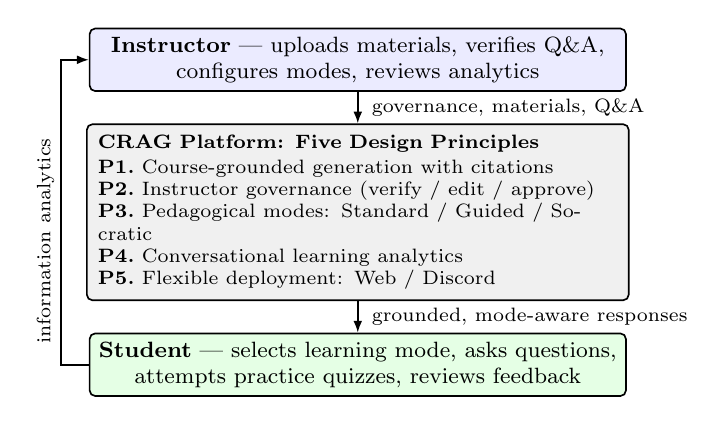
\begin{tikzpicture}[
  ibox/.style={rectangle, rounded corners=2pt, draw, semithick,
              fill=blue!8, align=center, text width=6.6cm, inner sep=3pt, font=\footnotesize},
  pbox/.style={rectangle, rounded corners=2pt, draw, semithick,
              fill=gray!12, align=left, text width=6.6cm, inner sep=4pt, font=\scriptsize},
  sbox/.style={rectangle, rounded corners=2pt, draw, semithick,
              fill=green!10, align=center, text width=6.6cm, inner sep=3pt, font=\footnotesize},
  arr/.style={-{Latex[length=1.5mm]}, semithick}
]
\node[ibox] (inst) {\textbf{Instructor} --- uploads materials, verifies Q\&A,\\configures modes, reviews analytics};
\node[pbox, below=4mm of inst] (plat) {\textbf{CRAG Platform: Five Design Principles}\\[1pt]
\textbf{P1.}~Course-grounded generation with citations\\
\textbf{P2.}~Instructor governance (verify / edit / approve)\\
\textbf{P3.}~Pedagogical modes: Standard / Guided / Socratic\\
\textbf{P4.}~Conversational learning analytics\\
\textbf{P5.}~Flexible deployment: Web / Discord};
\node[sbox, below=4mm of plat] (stud) {\textbf{Student} --- selects learning mode, asks questions,\\attempts practice quizzes, reviews feedback};
\draw[arr] (inst.south) -- node[right=0.5mm, font=\scriptsize]{governance, materials, Q\&A} (plat.north);
\draw[arr] (plat.south) -- node[right=0.5mm, font=\scriptsize]{grounded, mode-aware responses} (stud.north);
\draw[arr] (stud.west) -- ++(-0.35,0) coordinate(corner) |- (inst.west);
\node[anchor=center, rotate=90, font=\scriptsize, left=2mm] at ([yshift=30mm]corner) {information analytics};
\end{tikzpicture}
\caption{CRAG's design principles and interaction workflow.
Student interactions inform analytics for instructor review.}
\label{fig:framework}
\end{figure}

\section{System Implementation}
% Updated against docs/architecture/{01_high_level,04_upload_flow,10_query_processing,13_lms_answer_reviews}.md.
% Describes current source, not confirmation that every feature is deployed.

\subsection{Educational Features and Instructor Governance}
Instructors organise materials, review Q\&A and quizzes, and inspect cohort activity. Supplementary material is allowed for retrieval, but excluded from quiz generation and selection. Students ask questions, customise learning modes, and practice with quizzes. Learning modes have automatic mode switching to fit to the sentiment of the question.
The instructor LMS answer-review tab distinguishes \emph{Confirm}, \emph{Clarify} and \emph{Dismiss}. Confirm approves the original answer; Clarify supplies a reviewed answer and an explanation. Both create approved Q\&A and an in-app student inbox update. Dismiss records the review without creating approved Q\&A or an inbox message.

\subsection{Course-material Ingestion}
CRAG converts uploaded materials into Markdown to retain document structure, such as headings and lists. Selected visual regions, such as diagrams or images, are interpreted to produce searchable descriptions. The text is then divided and embedded into searchable passages. Answers are retrieved, generated, and supported with source citations for students to inspect.

\subsection{Query Handling}
Fig.~\ref{fig:workflow} shows the query flow. CRAG first identifies the selected learning mode and routes explicit
quiz requests to quiz generation. Other questions are embedded and checked against instructor-verified Q\&A at a similarity threshold of 0.85. A match returns the reviewed answer directly.
Otherwise, a Gemini planner judges course relevance and proposes complementary searches using recent conversation context. Clearly unrelated questions receive a course-scope response. Results are deduplicated and combined using reciprocal-rank fusion, with a default final context of five evidence items.

When retrieval signals suggest insufficient evidence, CRAG uses an automated review to identify missing information and may perform one additional search round. If no evidence is retrieved, it returns a fallback response; otherwise, it generates an answer using the selected learning mode, retrieved evidence and conversation history.

\begin{figure}[t]
\centering
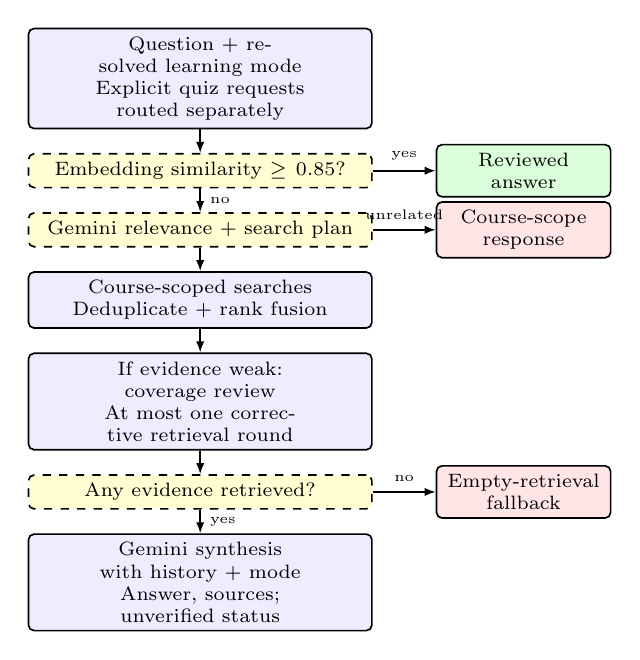
\begin{tikzpicture}[
 every node/.style={font=\scriptsize,align=center},
 proc/.style={rectangle,rounded corners=2pt,draw,semithick,fill=blue!7,text width=4.15cm,inner sep=3pt},
 dec/.style={proc,dashed,fill=yellow!18},
 outbox/.style={rectangle,rounded corners=2pt,draw,semithick,fill=green!14,text width=2.0cm,inner sep=3pt},
 arr/.style={-{Latex[length=1.4mm]},semithick}]
\node[proc] (q) {Question + resolved learning mode\\Explicit quiz requests routed separately};
\node[dec,below=3mm of q] (v) {Embedding similarity $\geq 0.85$?};
\node[outbox,right=8mm of v] (va) {Reviewed answer};
\node[dec,below=3mm of v] (p) {Gemini relevance + search plan};
\node[outbox,right=8mm of p,fill=red!10] (scope) {Course-scope\\response};
\node[proc,below=3mm of p] (r) {Course-scoped searches\\Deduplicate + rank fusion};
\node[proc,below=3mm of r] (c) {If evidence weak: coverage review\\At most one corrective retrieval round};
\node[dec,below=3mm of c] (e) {Any evidence retrieved?};
\node[outbox,right=8mm of e,fill=red!10] (empty) {Empty-retrieval\\fallback};
\node[proc,below=3mm of e] (g) {Gemini synthesis with history + mode\\Answer, sources; unverified status};
\draw[arr] (q) -- (v);
\draw[arr] (v) -- node[above,font=\tiny]{yes} (va);
\draw[arr] (v) -- node[right,font=\tiny]{no} (p);
\draw[arr] (p) -- node[above,font=\tiny]{unrelated} (scope);
\draw[arr] (p) -- (r);
\draw[arr] (r) -- (c);
\draw[arr] (c) -- (e);
\draw[arr] (e) -- node[above,font=\tiny]{no} (empty);
\draw[arr] (e) -- node[right,font=\tiny]{yes} (g);
\end{tikzpicture}
\caption{CRAG query-handling workflow.}
\label{fig:workflow}
\end{figure}

\section{Historical Evaluation}
\subsection{Controlled Behavioural Tests}
50 cases were scored pass/fail by a human judge, with learning mode and prompt configuration kept constant. Cases covered grounded answering, out-of-scope fallback, robustness and safety (Table~\ref{tab:controlled}). 
Reported failures included unnecessary refusals, unsupported
out-of-scope answers, difficulty handling ambiguous queries,
and compliance with adversarial or academic-misuse requests.
These findings illustrate limits of grounding and prompt-only
safeguards.

\begin{table}[t]
\centering
\caption{Controlled behaviour results for previous CRAG prototype.}
\label{tab:controlled}
\footnotesize
\begin{tabular}{@{}lcc@{}}
\toprule
\textbf{Category} & \textbf{Passed/tested} & \textbf{Pass rate} \\
\midrule
Grounding  & 8/10  & 0.80 \\
Fallback   & 9/10  & 0.90 \\
Robustness & 16/20 & 0.80 \\
Safety     & 6/10  & 0.60 \\
\midrule
Overall    & 39/50 & 0.78 \\
\bottomrule
\end{tabular}
\end{table}


\subsection{CS3247 Classroom Pilot}
A prior two-week CS3247 Game Development pilot (n=30) motivates the present needs assessment. The study comprised three phases: a pre-study survey on prior AI use and study habits; an interaction phase that logged CRAG conversations; and a post-study survey measuring perceived usefulness and trust on 5-point Likert scales. The pre-study showed majority relied on AI tools, and social barriers prevented help-seeking. The post-study reported interactions were mainly concept questions in Standard mode, with limited use of other modes. Query logs also revealed mismatches between student expectations and retrieval scope, such as (``what slides do you have access to'') or (``when are midterms''). Post-study responses indicated perceived gains in understanding and citation-related trust, alongside mixed views of overall reliability and usefulness relative to general-purpose AI. These were perceptions, not measured learning gains, and the 30 pilot participants should not be treated as the denominator for every survey item.

\section{CS3103 Assessment}
\subsection{Participants and Baseline Analysis}
Prior to utilising CRAG, all 110 eligible students enrolled in CS3103 (AY2026/27 Semester 1) were invited to provide research consent and complete a pre-study survey. A total of 42 students responded, yielding a response rate of 38.2\%, comprising 26 third-year (61.9\%) and 16 fourth-year (38.1\%) undergraduate students.
The survey analysed self-reported study habits, prior AI use, and preferences for educational AI assistants. Study-habit and expectation questions used a 5-point Likert scale ranging from \textit{Strongly Disagree} to \textit{Strongly Agree}. Agreement combines Agree and Strongly Agree, while other items used categorical choices, multiple selections or optional open-text responses. Multiple-selection percentages use respondents as denominators and may sum above 100\%. 
This analysis provides a baseline for investigating whether and how students' subsequent CRAG interactions exhibit HCD-related behaviours, including creation, critique and reflection, throughout the semester; these responses are not confirmed CRAG users, as the survey was conducted prior to any interaction with the platform.


\subsection{Prior Habits and Desired Support}
Table~\ref{tab:cs3103baseline} summarises selected baseline findings. High frequencies of general AI utilisation and reported follow-up querying behaviours strongly motivate the need to study multi-turn student interactions. The distribution of self-declared messages per conversation was 1--3 messages for 3/41 respondents (7.3\%), 4--6 messages for 18/41 (43.9\%), 7--9 messages for 5/41 (12.2\%), and more than 10 messages for 15/41 (36.6\%). While these categorical ranges preclude the calculation of an exact mean and do not equate to empirically observed conversational turns, they highlight a clear student tendency toward extended dialogues. Furthermore, factual recall was the primary query type for 12/41 respondents (29.3\%), followed closely by summarisation or step-by-step breakdowns for 11/41 respondents (26.8\%), with the remaining pool selecting conceptual checking or critical analysis. Crucially, these distributions map baseline student preferences and reported habits rather than active, empirically verified HCD processes.

\begin{table}[t]
\centering
\caption{CS3103 pre-use survey: selected self-reported habits and preferences. Denominators exclude missing answers.}
\label{tab:cs3103baseline}
\footnotesize
\setlength{\tabcolsep}{3pt}
\begin{tabular}{@{}p{5.1cm}rr@{}}
\toprule
Finding & Count & \% \\
\midrule
Uses AI often or always for studying & 35/42 & 83.3 \\
Clarifying follow-up after unclear AI answer & 32/41 & 78.0 \\
At least four prompts per conversation & 38/41 & 92.7 \\
Stops when able to explain concept\textsuperscript{a} & 36/41 & 87.8 \\
Most frequent query: checking understanding & 12/41 & 29.3 \\
Most frequent query: critical analysis & 6/41 & 14.6 \\
Wants instructor-verified answers\textsuperscript{a} & 33/41 & 80.5 \\
Wants exact-slide citations\textsuperscript{a} & 31/41 & 75.6 \\
Wants strict course grounding\textsuperscript{a} & 26/41 & 63.4 \\
\bottomrule
\end{tabular}
\par\smallskip
\parbox{\columnwidth}{\footnotesize\textsuperscript{a}Multiple-selection item; selecting conceptual explainability does not demonstrate that understanding was achieved.}
\end{table}

\subsection{Design Implications}
The baseline supports three design priorities. First, reported follow-up behaviour makes continuity across questions important: course evidence should remain available as students clarify or revise an explanation. Longer conversations can also reflect confusion, repeated failures or task complexity, so their length, by itself, cannot establish productive engagement.
Second, preferences for instructor verification and source citations motivate inspectable answers and review workflows. The current corrective pipeline attempts to improve evidence coverage, but its effectiveness is not yet evaluated.
Third, demand for step-by-step explanation should not be conflated with a preference for hint-only interaction. Students may seek a direct explanation at one point and a challenge to their reasoning at another. Offering multiple modes is a design response to this variation; actual mode uptake, usefulness and instructional effects require observation.

\subsection{An iterative HCD study}
We propose extending CRAG's assistance to the HCD cycle~\cite{b_hcd}. Students would state an initial idea, critically compare CRAG's output against current evidence, and justify a reason. AI feedback should support this process while students retain responsibility for accepting, rejecting and explaining suggestions.
The CS3103 baseline makes this distinction concrete: respondents report sustained conversations and understanding-oriented stopping criteria, but the survey does not test their explanations or revisions. A subsequent study must examine student-generated evidence rather than infer reflection from prompt counts.
The research question is: how do students use course-grounded AI feedback to reflect on, critique and revise their own work? The evidence should link initial reasoning, feedback, and subsequent revision, while analysis should follow participants across observations and avoid treating multiple messages from one student as independent participants. Instructor studies should examine presence of reasoning tasks in conversations, and how analytics influence feedback.


\section{Discussion}

\subsection{Strict Grounding versus Generative Flexibility}
The prototype findings suggest a tension between students' expectations of flexible explanation and instructors' need for course alignment and accountability. Over-conservative refusals and requests beyond literal slide content motivated closer attention to evidence coverage. The current implementation expands on weak coverage by generating a personalised answer using the pool of relevant sources found.

\subsection{Controlled Correctness versus Experienced Usefulness}
Controlled tests and user reports answer different questions. The historical suite measured behaviour on 50 selected cases; the pilot survey described perceived usefulness. Neither establishes learning gains, superiority over general-purpose assistants or current-system performance. Citation preferences do not show that cited passages support claims. Future evaluation should examine source location, claim support and citation coverage separately, alongside instructor review workload and student use of later clarifications.

\section{Limitations and Future Work}
The historical study covered two weeks, two lectures and one course at one institution. Outcomes were self-reported, without objective knowledge assessments. Standard-mode dominance limits conclusions about other modes. Post-survey item denominators, ethics arrangements and study procedures require confirmation from original records.

Current source includes selective visual ingestion, adaptive modes, corrective retrieval and LMS answer reviews, but historical results cannot validate these additions. LLM safety still remains an open research problem. Freeze the current corpus, build, model settings and scoring criteria; compare standard RAG and corrective retrieval on the same questions, including unsupported answers, benign queries, direct and document-borne prompt injection, and course-defined academic misuse. Report category counts and independent judge agreement.

CRAG prioritises consent-eligible capture, response provenance, deterministic exports, independently validated coding and learner-authored work. A longitudinal study should link initial reasoning, AI feedback and justified revision, with independent or delayed outcomes. Conversation length, mode selection and cognitive annotations alone do not demonstrate learning. Operational logs must not automatically become research data; approval, consent, access and retention arrangements require explicit verification.

The separate access-control release remains deferred and is not part of the current implementation. Its protections must not be claimed as deployed. Ordinary-upload recovery and durable ingestion workers also remain future work. Selective PDF visual processing is already implemented; extending support to recordings or other media remains distinct from validating this existing capability. Browser workflows, applied migrations and live deployment require checks beyond source inspection.

\section{Conclusion}
CRAG integrates course grounding, instructor review, pedagogical modes and analytics. It uses a Gemini planner for weaker questions, bounded corrective retrieval, and LMS question updates. These design concerns are motivated by historical survey and usage, but current technical reliability, safety and educational effectiveness require a new, version-specific evaluation.
\section*{Acknowledgment}
The authors thank Assoc.\ Prof.\ Anand Bhojan for supervision, and the CS3247 students who participated in the study.

\begin{thebibliography}{00}
\bibitem{b_yayeh} Y.~Yayeh, W.~Admass, Y.~B. Chekol, A.~M. Mekonnen, and M.~Asmare, ``ChatGPT in education: A systematic review on opportunities, challenges, and future directions,'' \emph{Algorithms}, vol.~18, no.~6, art.~352, 2025.
\bibitem{b_bender} E.~M. Bender, T.~Gebru, A.~McMillan-Major, and S.~Shmitchell, ``On the dangers of stochastic parrots: Can language models be too big?,'' in \emph{Proc.\ ACM Conf.\ on Fairness, Accountability, and Transparency (FAccT)}, 2021, pp.~610--623.
\bibitem{b_heersmink} R.~Heersmink, B.~de Rooij, M.~J. Clavel V\'azquez, and M.~Colombo, ``A phenomenology and epistemology of large language models: Transparency, trust, and trustworthiness,'' \emph{Ethics Inf.\ Technol.}, vol.~26, no.~3, 2024.
\bibitem{b_delikoura} I.~Delikoura, Y.~R. Fung, and P.~Hui, ``From superficial outputs to superficial learning: Risks of large language models in education,'' arXiv:2509.21972, 2025.
\bibitem{b_lewis} P.~Lewis \emph{et~al.}, ``Retrieval-augmented generation for knowledge-intensive NLP tasks,'' in \emph{Adv.\ Neural Information Processing Systems (NeurIPS)}, 2020.
\bibitem{b_gao_citations} T.~Gao, H.~Yen, J.~Yu, and D.~Chen, ``Enabling large language models to generate text with citations,'' in \emph{Proc.\ Conf.\ on Empirical Methods in Natural Language Processing (EMNLP)}, 2023, pp.~6465--6488, doi: 10.18653/v1/2023.emnlp-main.398.
\bibitem{b_autotutor} A.~C. Graesser, K.~Wiemer-Hastings, P.~Wiemer-Hastings, and R.~Kreuz, ``AutoTutor: A simulation of a human tutor,'' \emph{Cogn.\ Syst.\ Res.}, vol.~1, no.~1, pp.~35--51, 1999.
\bibitem{b_chi} M.~T.~H. Chi, N.~de Leeuw, M.-H. Chiu, and C.~LaVancher, ``Eliciting self-explanations improves understanding,'' \emph{Cogn.\ Sci.}, vol.~18, no.~3, pp.~439--477, 1994.
\bibitem{b_ferguson} R.~Ferguson, ``Ethical challenges for learning analytics,'' \emph{J.\ Learn.\ Anal.}, vol.~6, no.~3, 2019.
\bibitem{b_hcd} A.~Bhojan, ``Pedagogical reflections on the Holistic Cognitive Development (HCD) framework and AI-augmented learning in creative computing,'' arXiv:2511.06779v2, Jan.~2026, doi: 10.48550/arXiv.2511.06779.
\bibitem{b_jillwatson} A.~K. Goel and L.~Polepeddi, ``Jill Watson: A virtual teaching assistant for online education,'' in \emph{Learning Engineering for Online Education}, C.~Dede \emph{et~al.}, Eds.\ Routledge, 2018, pp.~120--143.
\end{thebibliography}

\end{document}
